\chapter{Completeness analysis}
\label{chapter:cad}

Figure~\ref{fig:l2cad-fm1} to Figure~\ref{fig:l2cad-fm24}
show the amount af available Level1B data and succesfully
processed Level2 data by month for the considered FreqModes.
The amount of available Level1B data varies during mission.
During the first six years of the mission \smr\ was operated
both in aeronomy and astronomy mode, and hence less
aeronomy observations are available for these years
compared to after 2008.  
During the most recent years \smr\ has both partly and completely
been turned off during the summer month.

FreqMode 1 and 2 (not yet fully processed and Figure is missing)
are the most applied modes, and 5000-10000 scans have been
observed each month. Level2 processing have been succesfully
for the majority of the available Level1B data.

FreqMode 14, 22, 24 are deployed for \chem{CO} observations.
The frontend used for these observations have been unstable
(drifting in frequency), and that can result in that the 
\chem{CO} signature is not covered in observed spectra 
of some of the scans. This gives that the fraction of
sussessful level2 processing is lower for these modes
compared to the others.
 
More text here...




\begin{figure}[t]
\centering
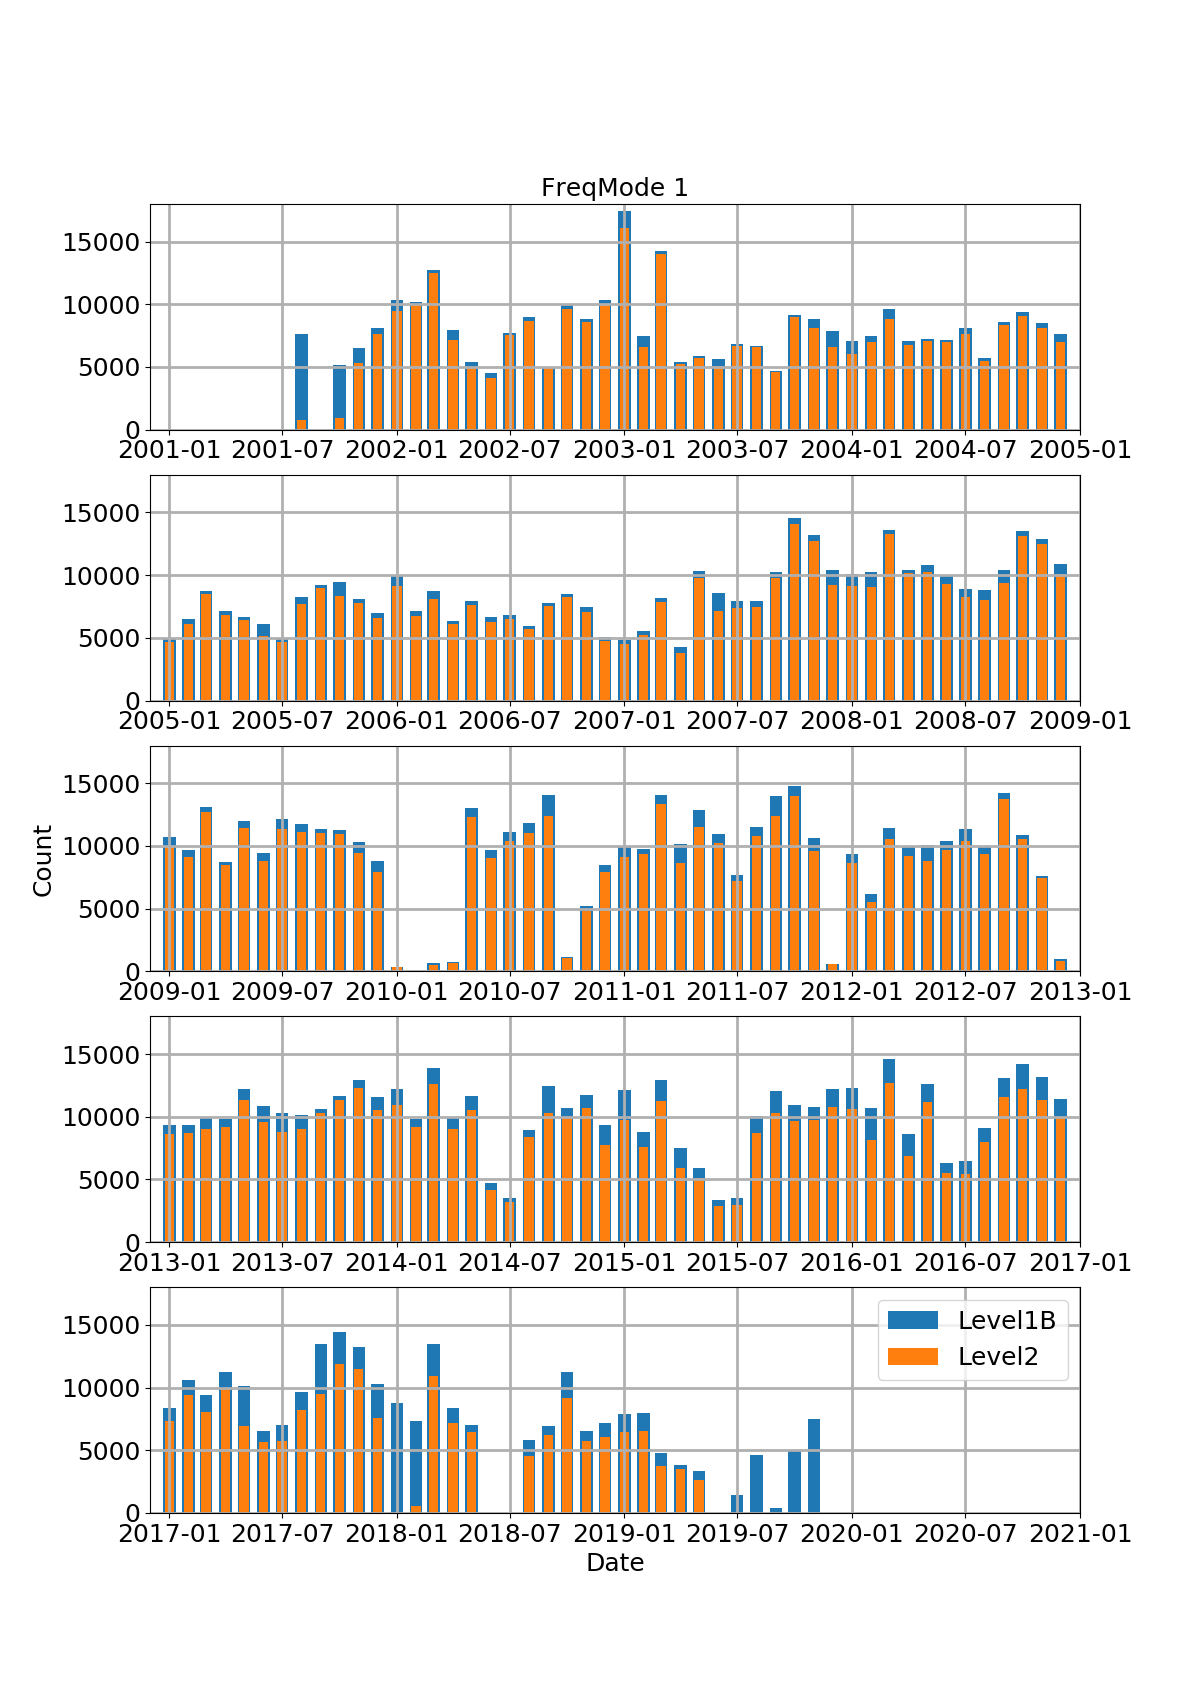
\includegraphics[width=1.0\textwidth]{l2cad-fm1.png}
\caption{Number of available Level1b and succesfully processed Level2
scans by month for FreqMode 1, during the complete \smr\ mission.}
\label{fig:l2cad-fm1}
\end{figure}

\begin{figure}[t]
\centering
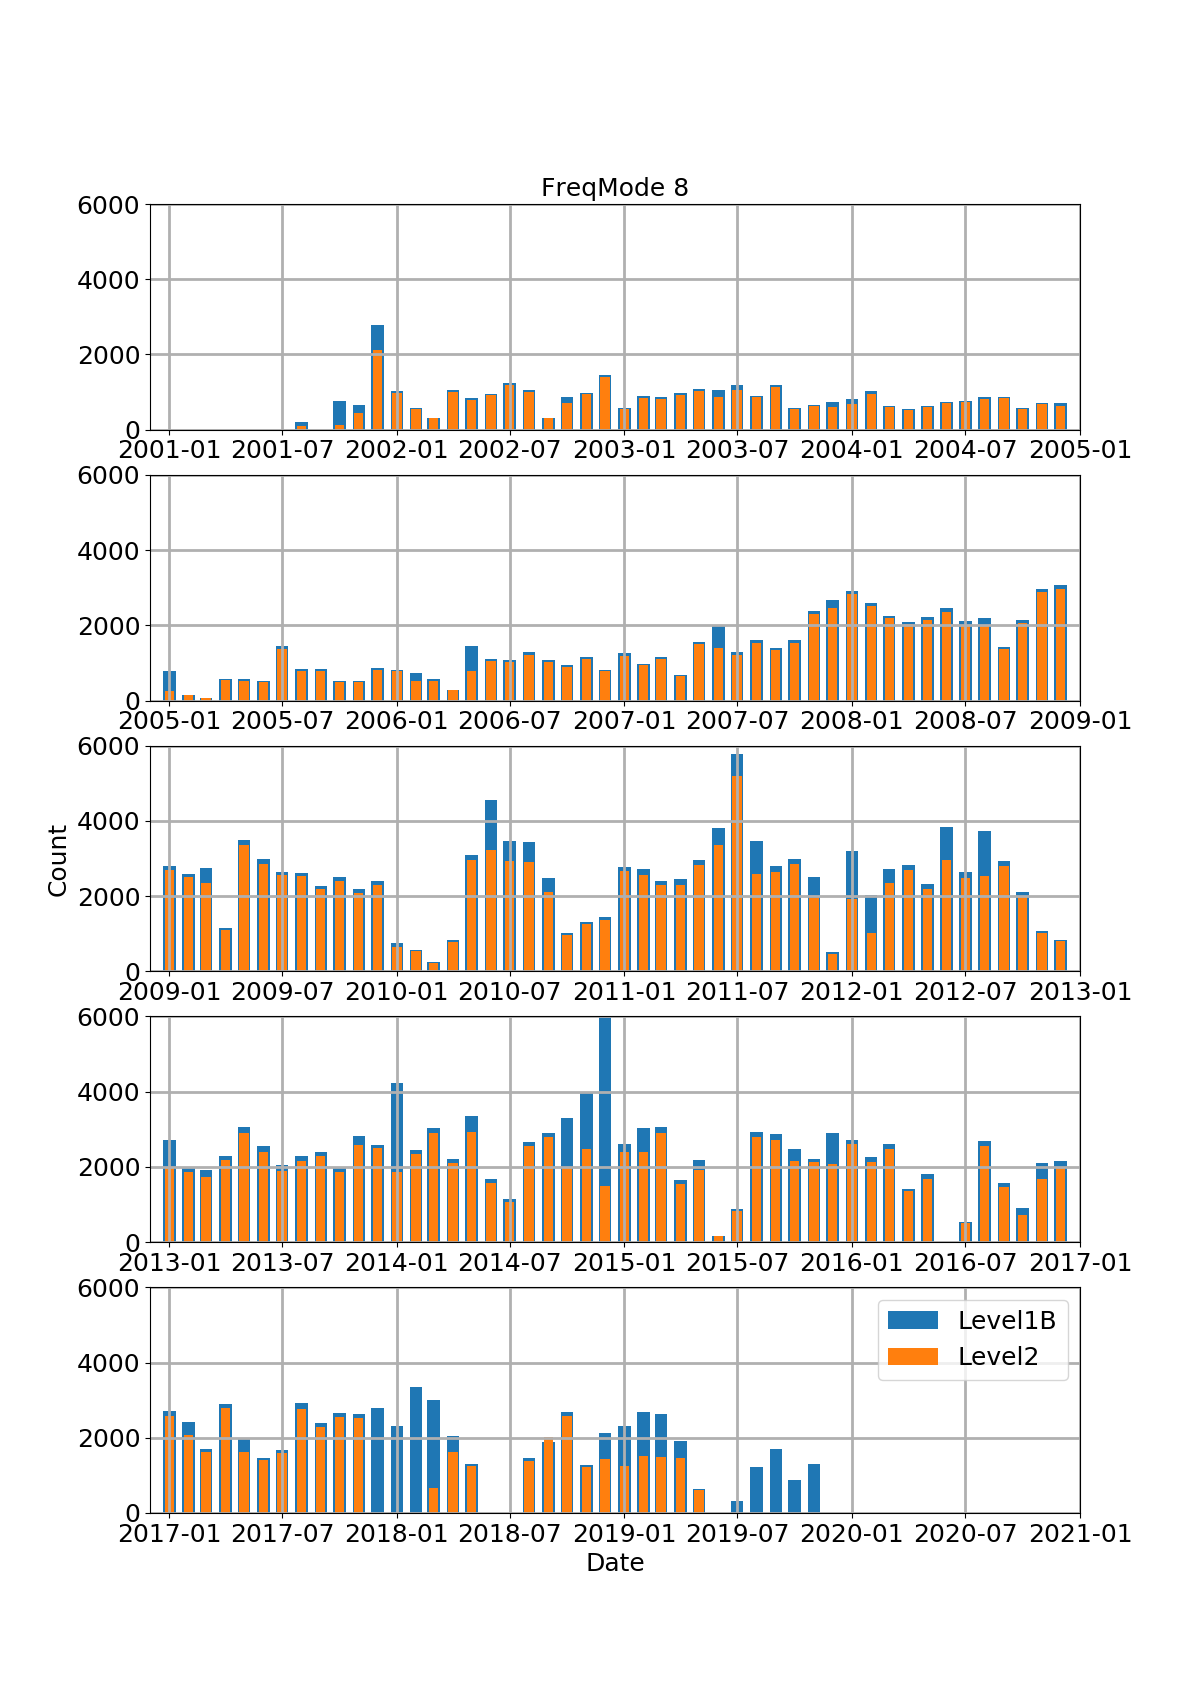
\includegraphics[width=1.0\textwidth]{l2cad-fm8.png}
\caption{As Figure~\ref{fig:l2cad-fm1} but for FreqMode 8.}
\label{fig:l2cad-fm8}
\end{figure}

\begin{figure}[t]
\centering
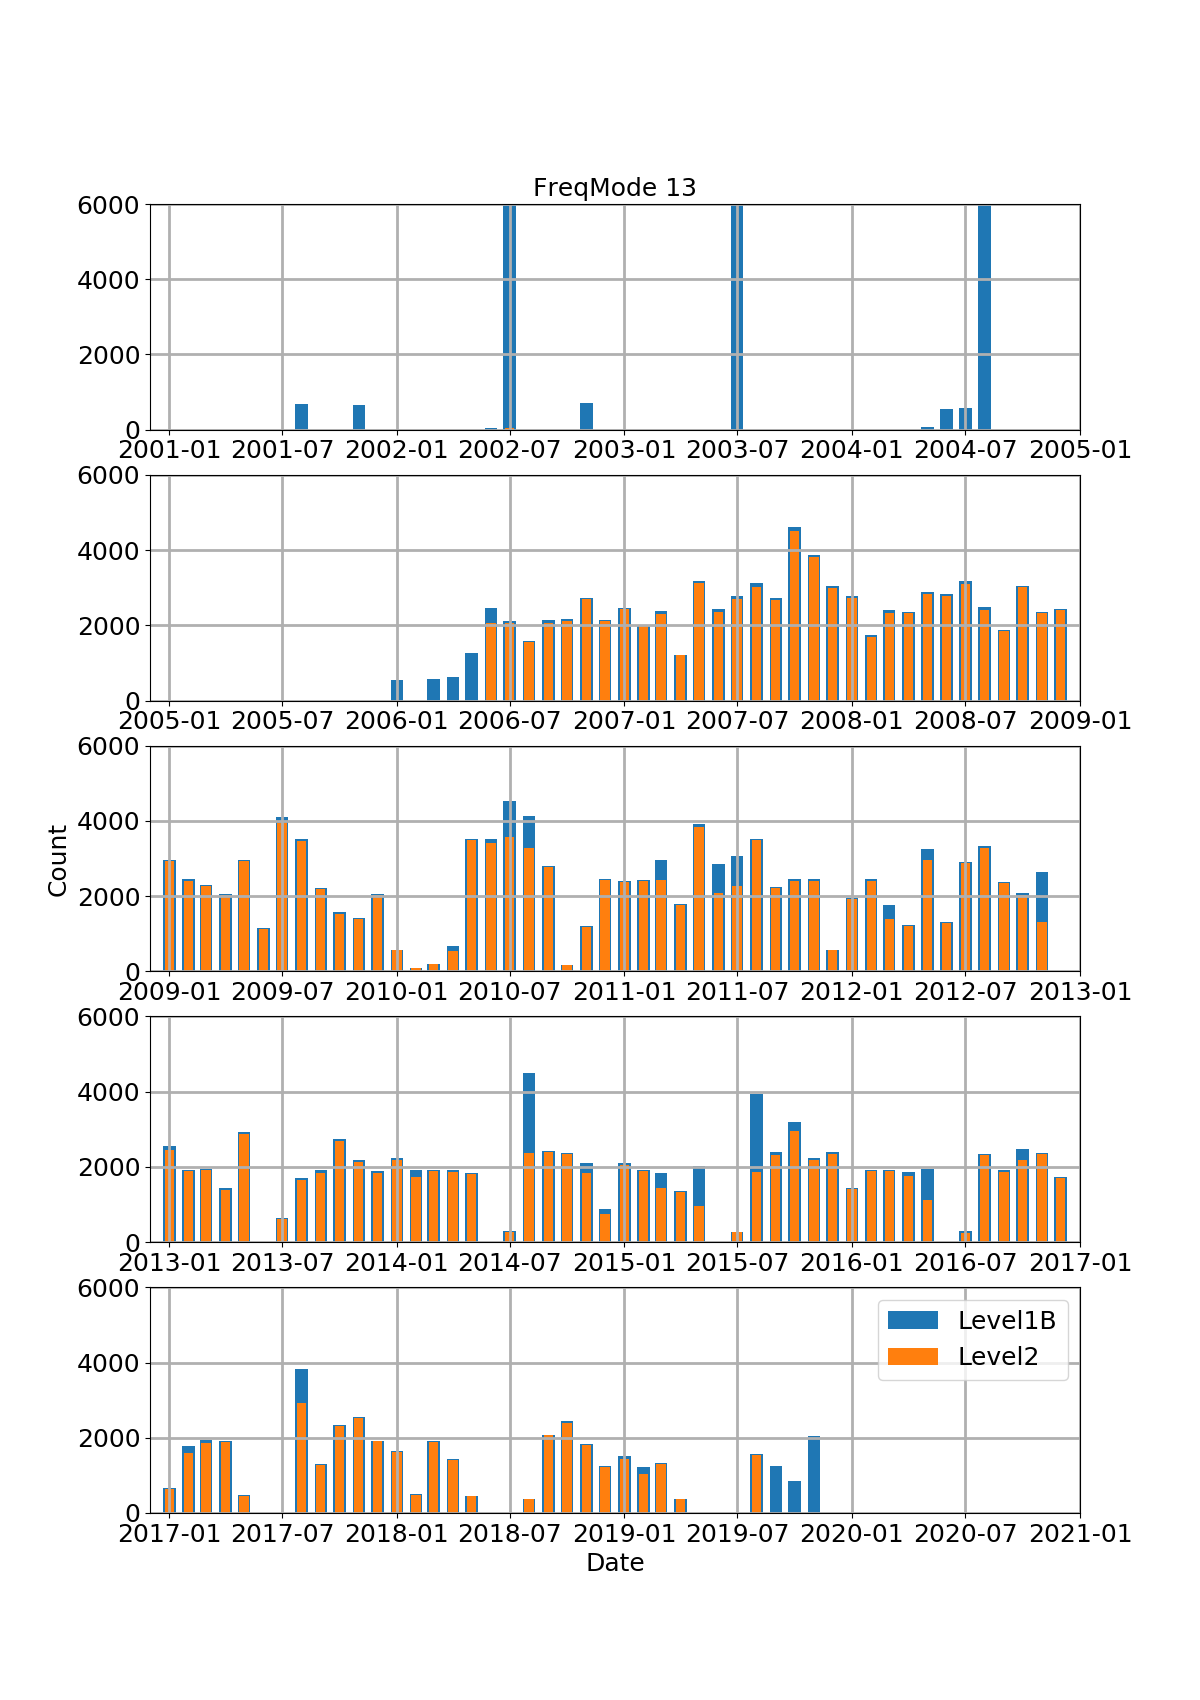
\includegraphics[width=1.0\textwidth]{l2cad-fm13.png}
\caption{As Figure~\ref{fig:l2cad-fm1} but for FreqMode 13.}
\label{fig:l2cad-fm13}
\end{figure}

\begin{figure}[t]
\centering
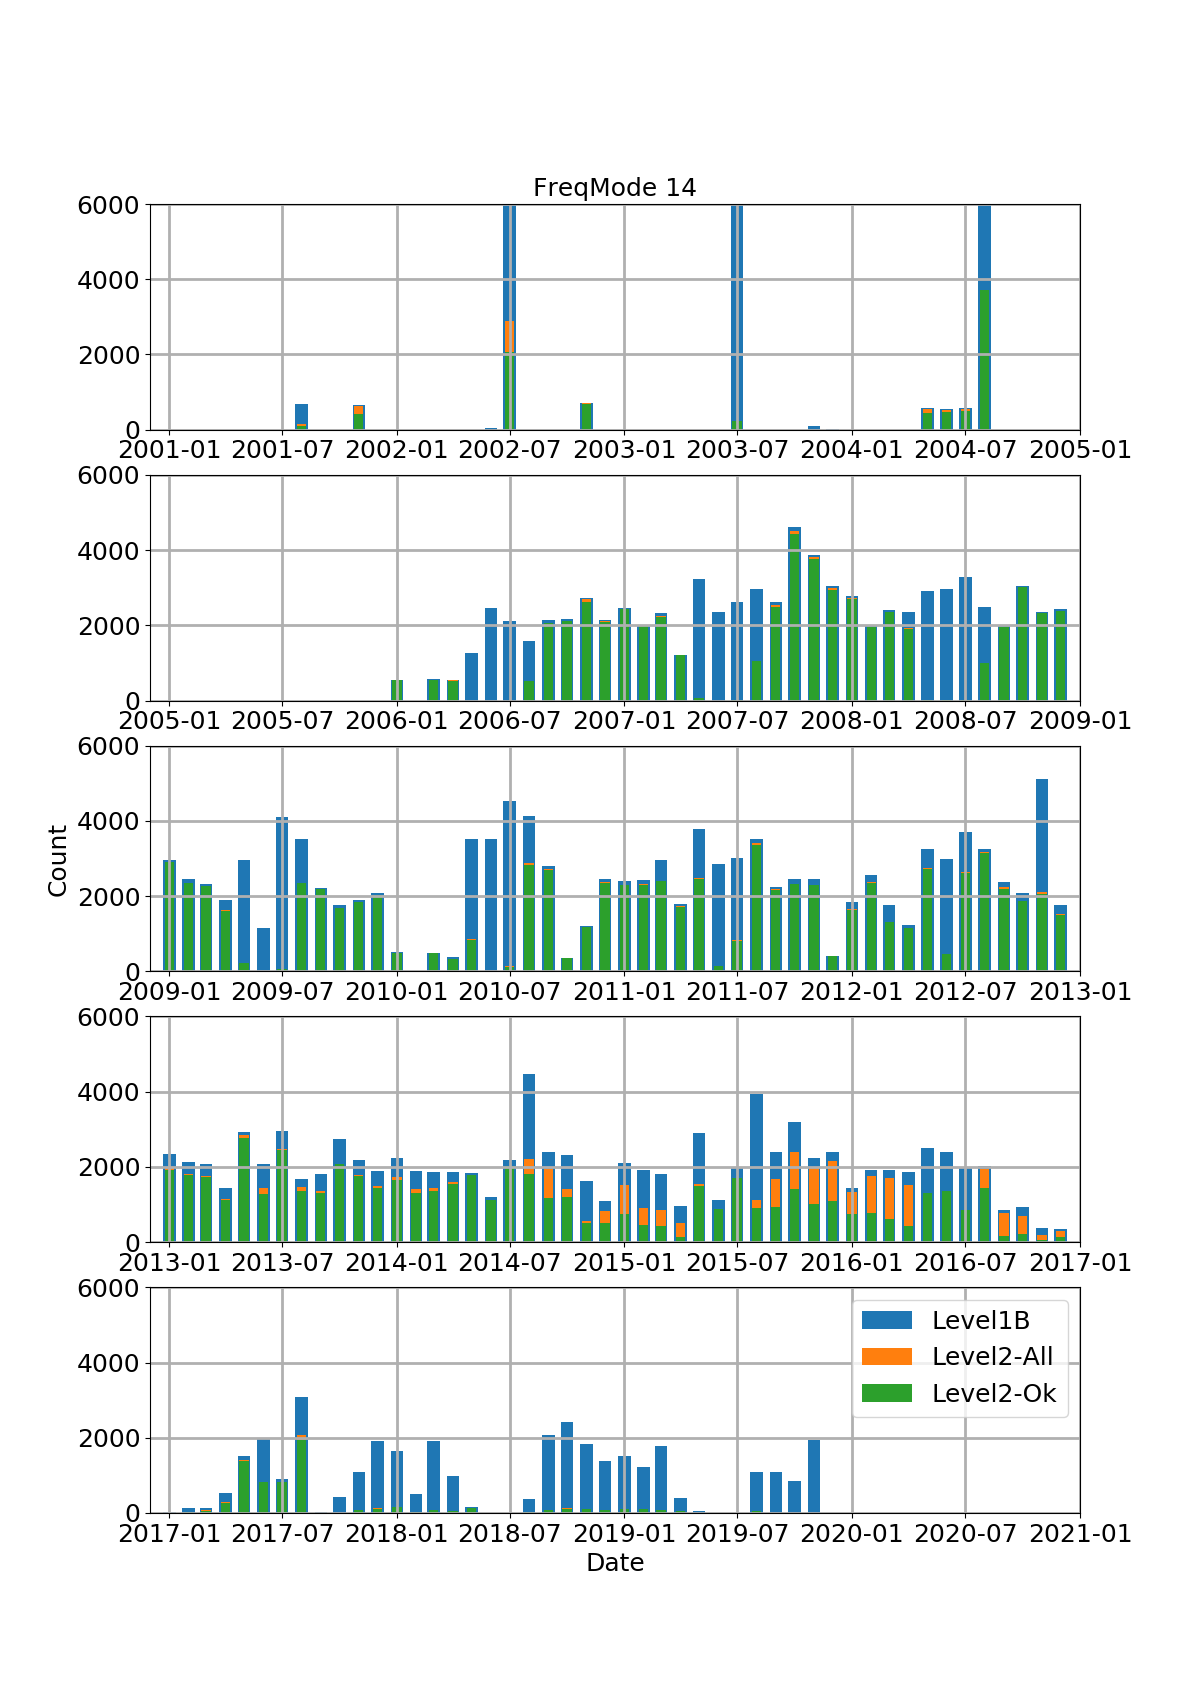
\includegraphics[width=1.0\textwidth]{l2cad-fm14.png}
\caption{As Figure~\ref{fig:l2cad-fm1} but for FreqMode 14.}
\label{fig:l2cad-fm14}
\end{figure}

\begin{figure}[t]
\centering
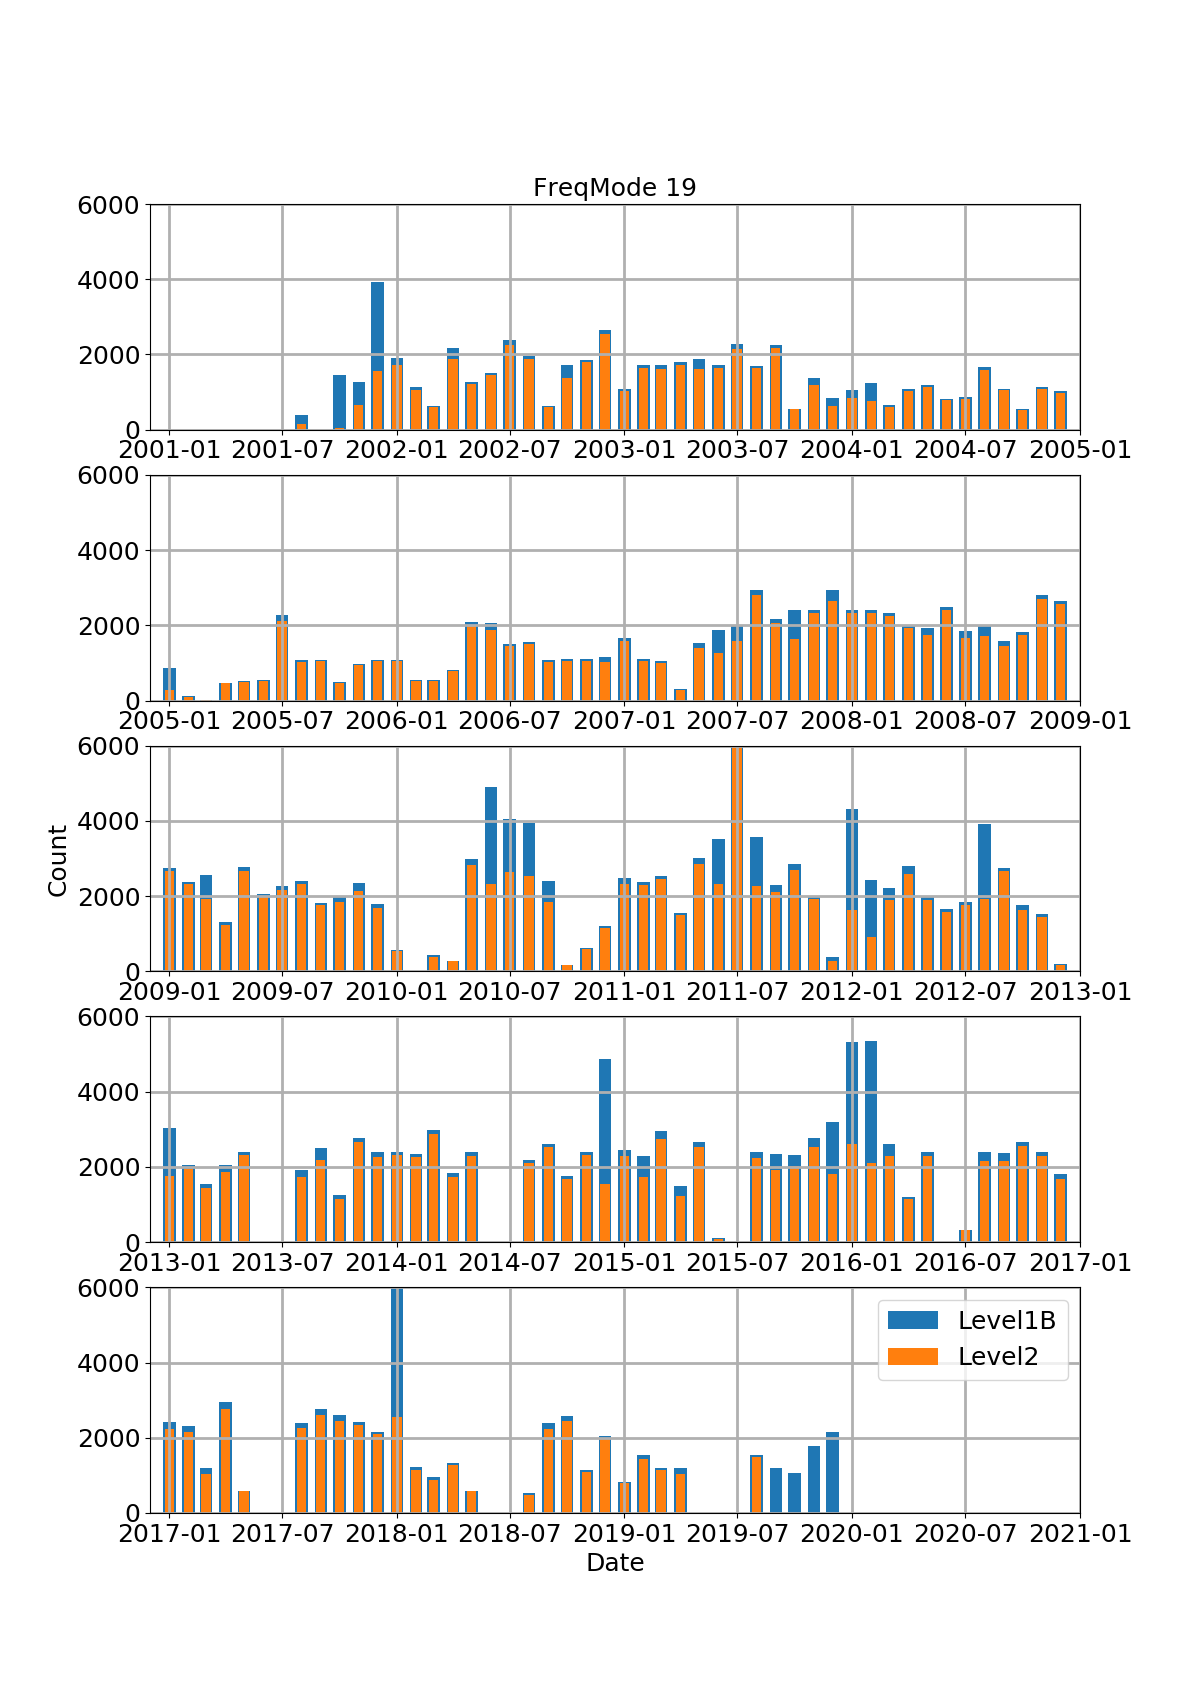
\includegraphics[width=1.0\textwidth]{l2cad-fm19.png}
\caption{As Figure~\ref{fig:l2cad-fm1} but for FreqMode 19.}
\label{fig:l2cad-fm19}
\end{figure}

\begin{figure}[t]
\centering
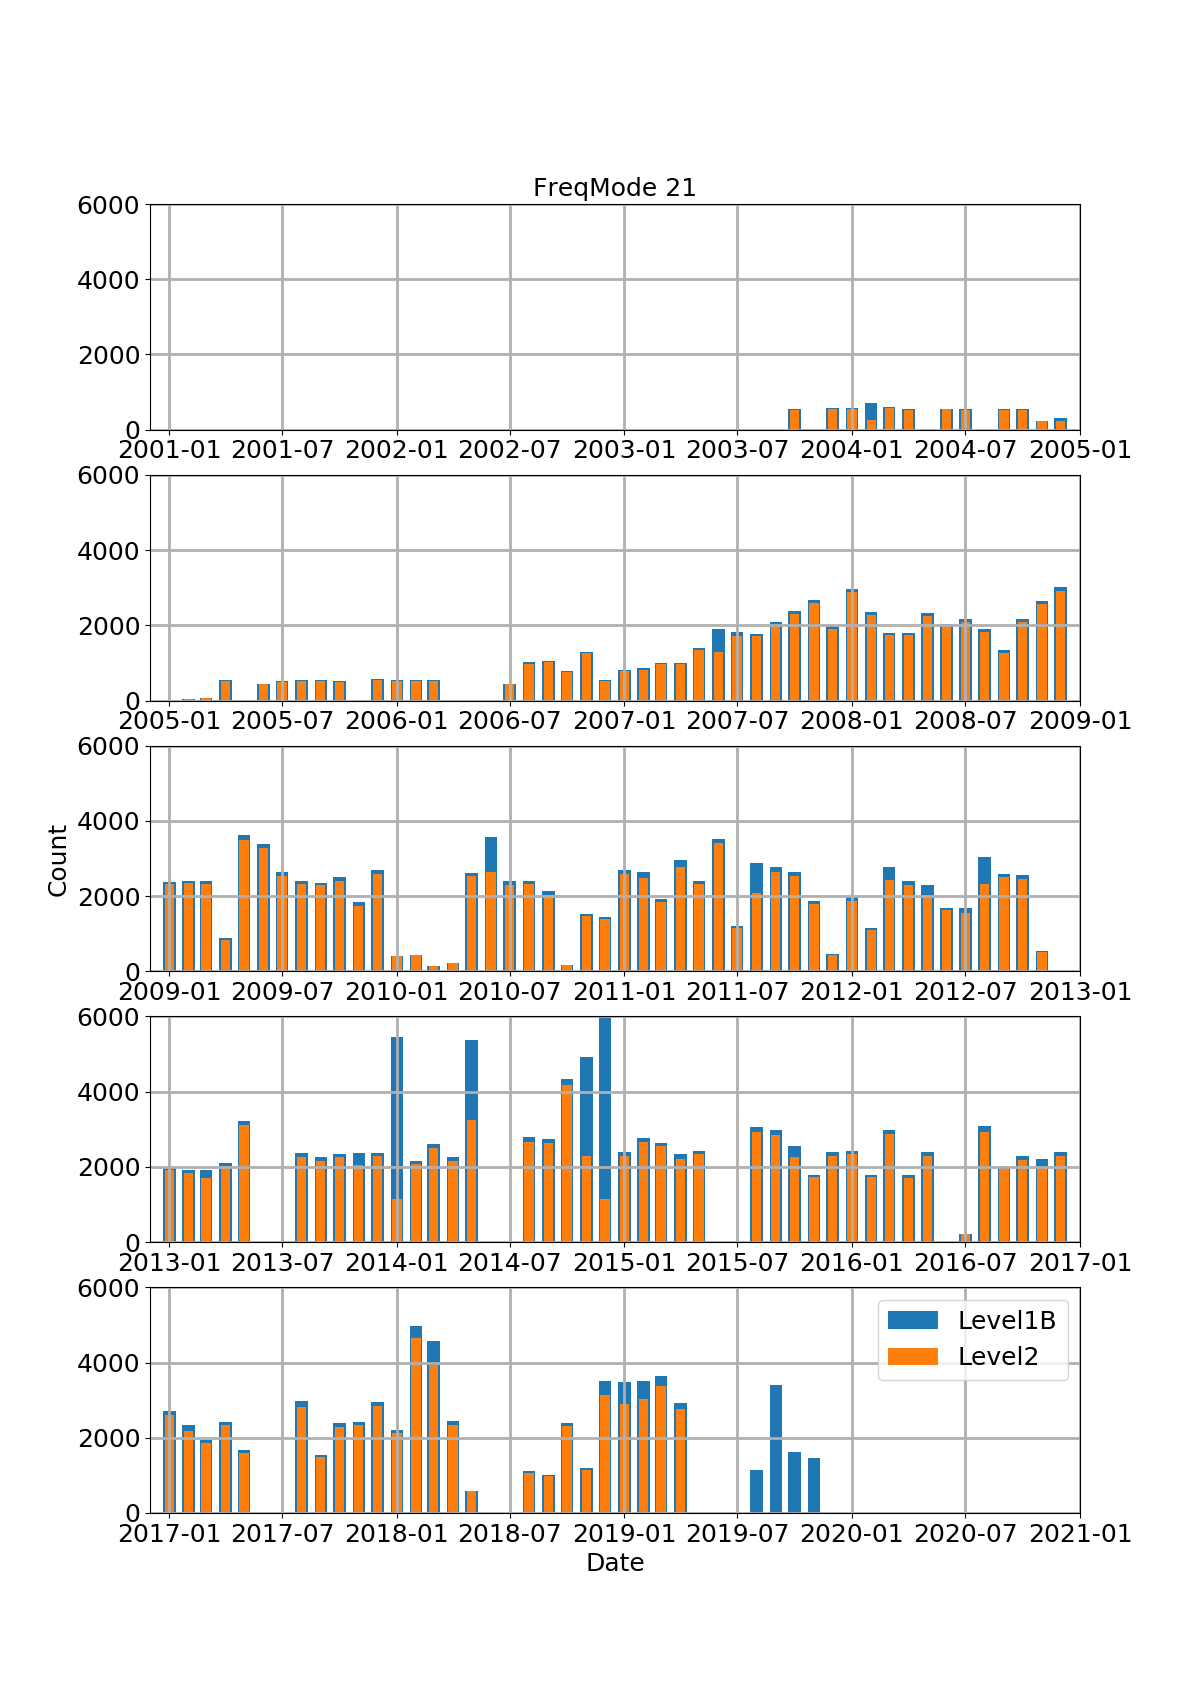
\includegraphics[width=1.0\textwidth]{l2cad-fm21.png}
\caption{As Figure~\ref{fig:l2cad-fm1} but for FreqMode 21.}
\label{fig:l2cad-fm21}
\end{figure}

\begin{figure}[t]
\centering
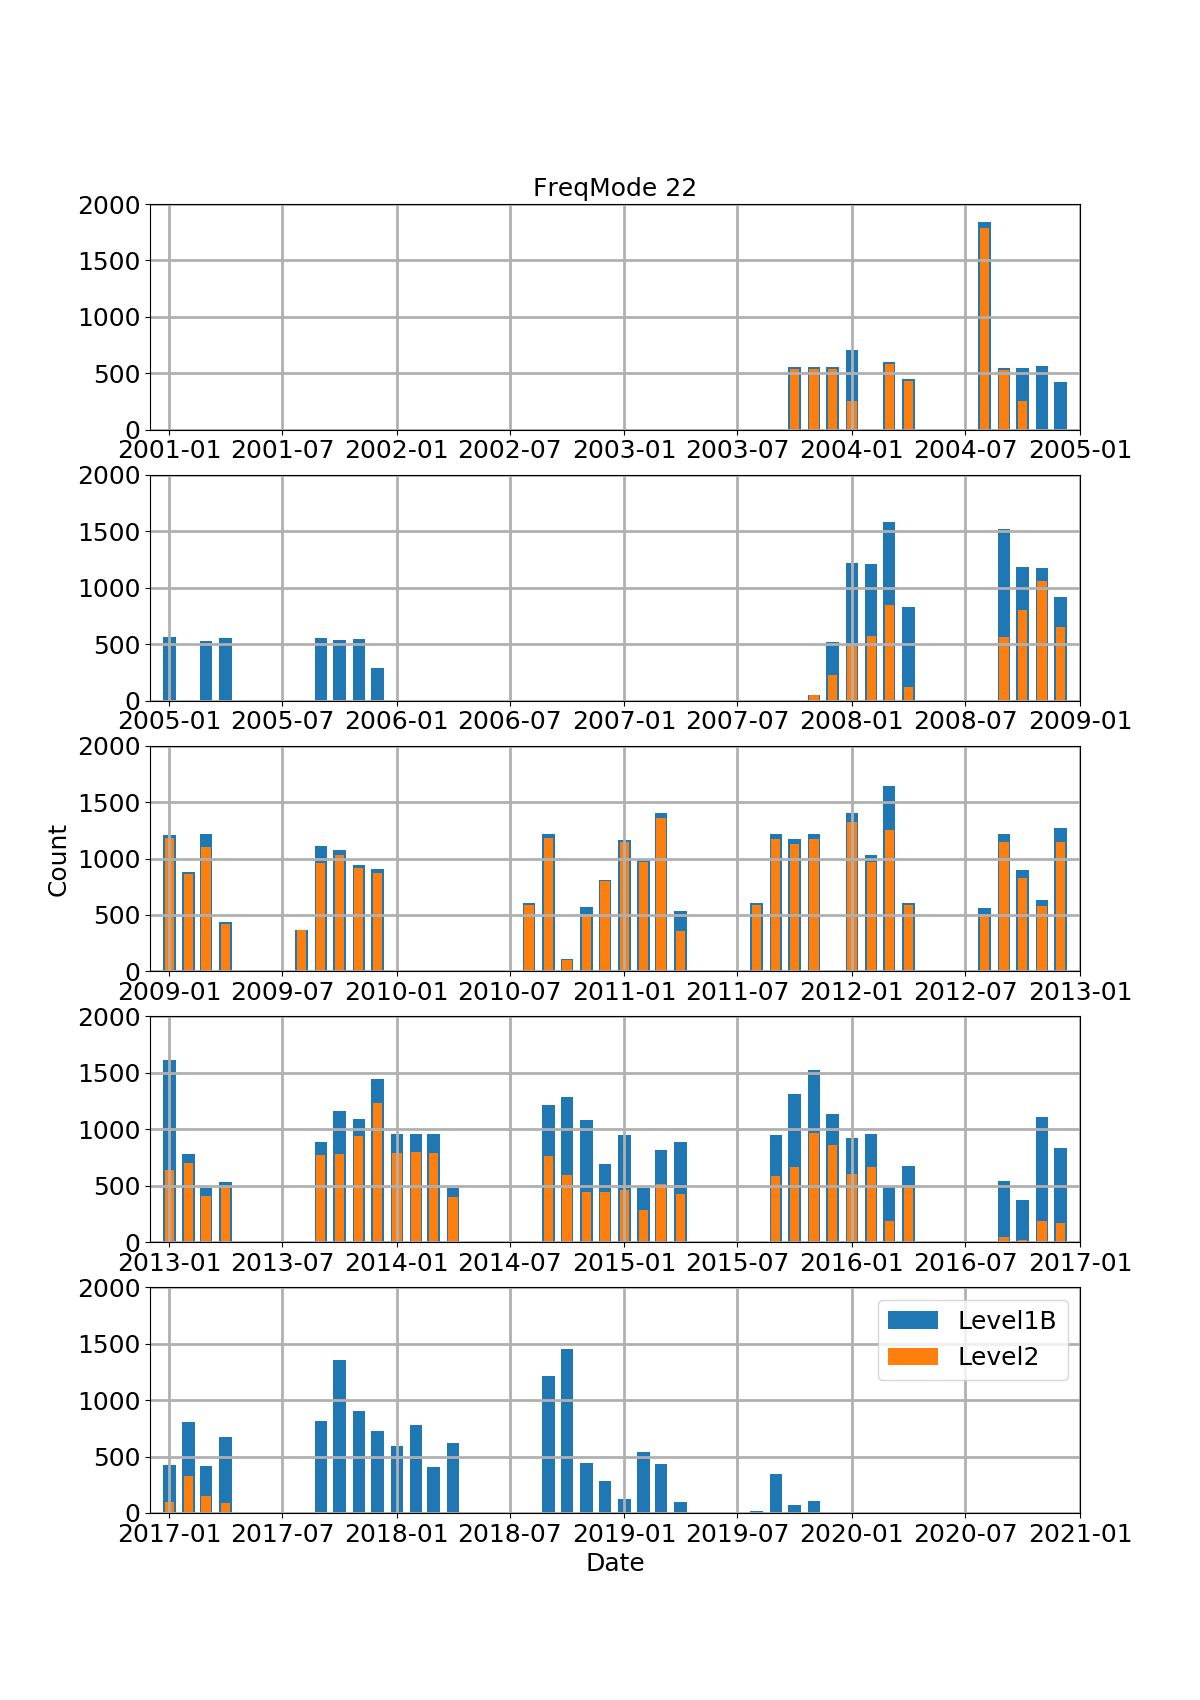
\includegraphics[width=1.0\textwidth]{l2cad-fm22.png}
\caption{As Figure~\ref{fig:l2cad-fm1} but for FreqMode 22.}
\label{fig:l2cad-fm22}
\end{figure}

\begin{figure}[t]
\centering
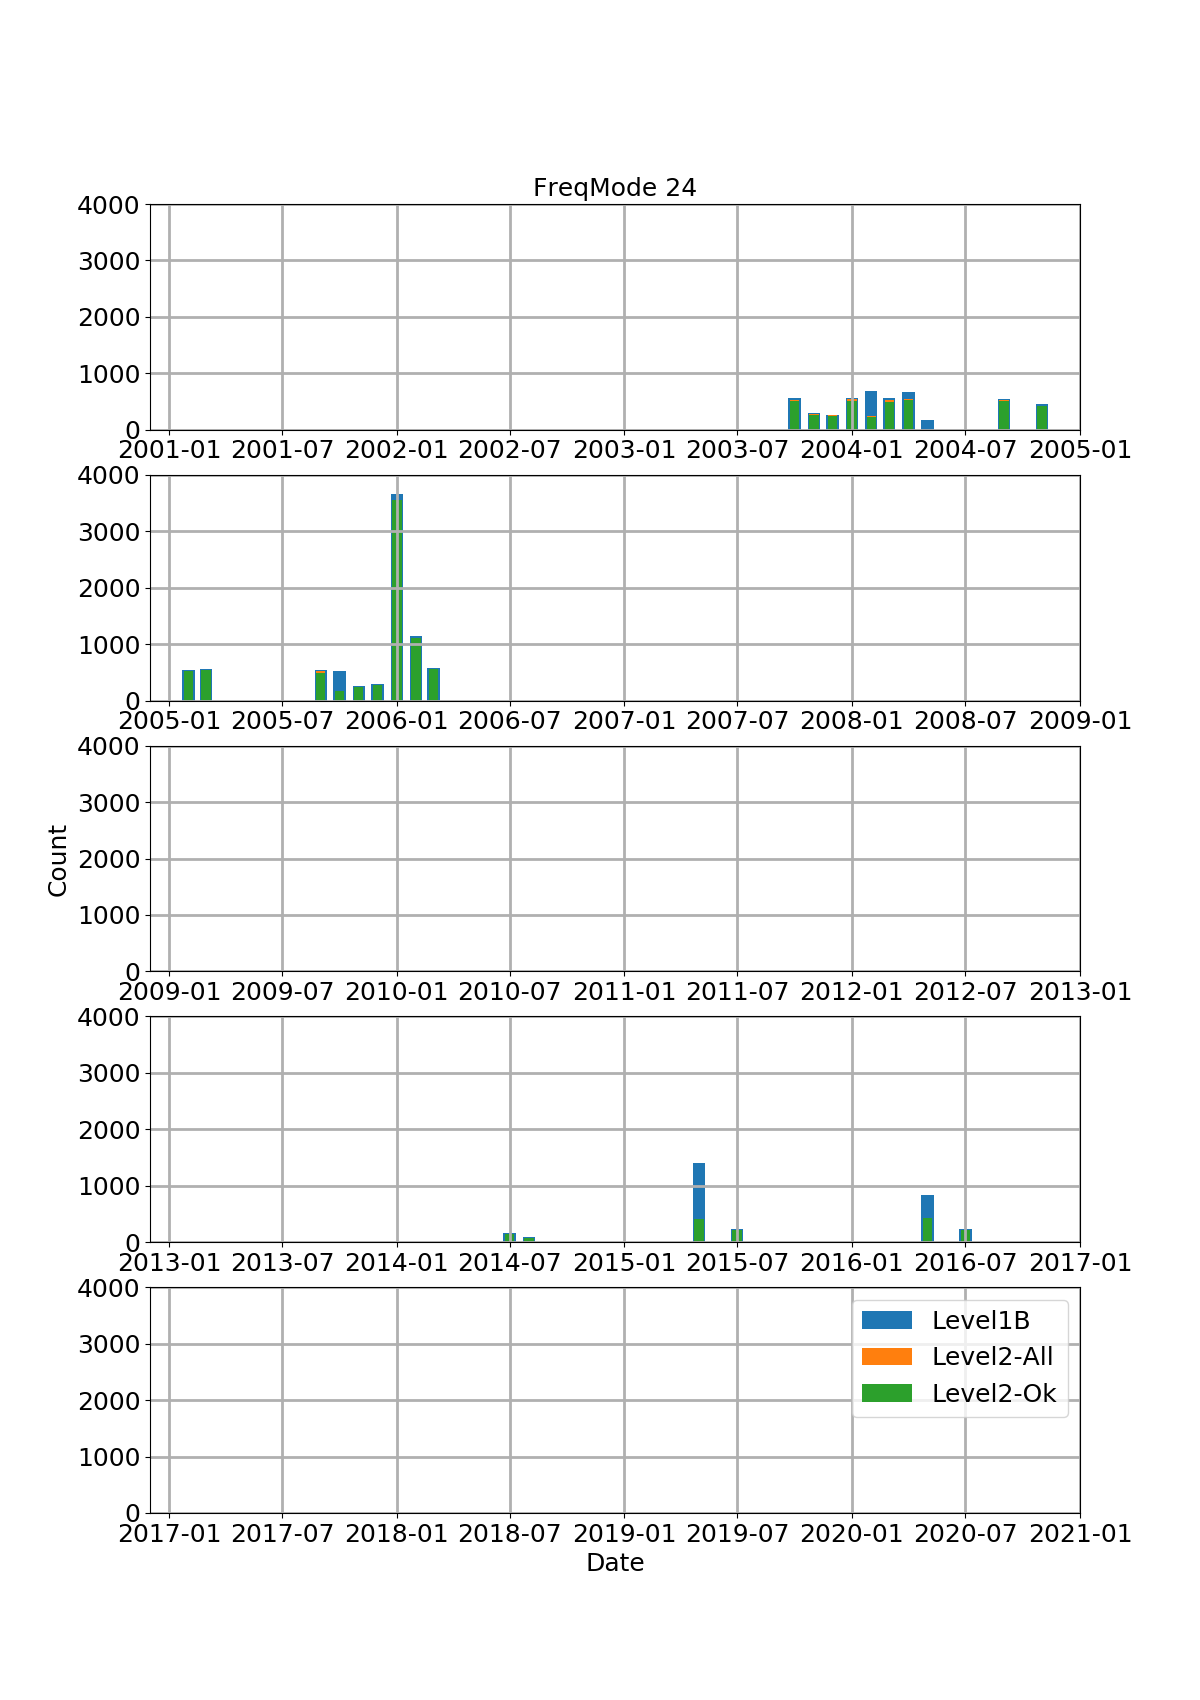
\includegraphics[width=1.0\textwidth]{l2cad-fm24.png}
\caption{As Figure~\ref{fig:l2cad-fm1} but for FreqMode 24.}
\label{fig:l2cad-fm24}
\end{figure}
